%&"../net"
\endofdump
\tikzexternalize[prefix=cache/]{lab05}
% https://shimo.im/docs/xJTTRDH6YrkcvvTG/read
\begin{document}
    \title{Write SDN Controller}
    \maketitle
    \tableofcontents
    \vfill
    Ryu provides software components with well defined API's that make it easy for developers to create new network management and control applications.
    \vfill
    \clearpage
    \section{建立网络}
    Set up the following network first:
    
    \hfill
    \begin{tikzpicture}
    \tikzstyle{host}=[draw]
    \tikzstyle{switch}=[draw]
    \tikzstyle{connection}=[]
    \tikzstyle{constr}=[right,font=\ttfamily\small]
    
\node (h1) [host] at (-0.5,0.5) {h1};
\node (s1) [switch] at (1.5,0.5) {s1};
\node (s3) [switch] at (3,2) {s3};
\node (s2) [switch] at (4.5,0.5) {s2};
\node (s4) [switch] at (3,-1) {s4};
\node (h2) [host] at (6.5,0.5) {h2};
\draw  (h1) edge (s1);
\draw  (s1) edge (s3);
\draw  (s3) edge (s2);
\draw  (s2) edge (s4);
\draw  (s4) edge (s1);
\draw  (s2) edge (h2);
\end{tikzpicture}

    使用给出的示例代码。但是为了处理上的方便,将会指定链路连接的端口号。
    \code{loopnet.py}

    \section{定时切换}
    Write an RYU controller that switches paths (h1-s1-s3-s2-h2 or h1-s1-s4-s2-h2) between h1 and h2 every 5 seconds. 

    查看修改流的定义函数。其中参数 \texttt{hard\_timeout} 用于定义丢弃流前的最大秒数。

    \codeseg{../ryu/ryu/ofproto/ofproto\_v1\_3\_parser.py}{2703}{2710}
    
    参数 \texttt{flags} 可以被指定为 \texttt{OFPFF\_SEND\_FLOW\_REM},可以用于在丢弃流后发出事件用于相关处理。

    \begin{quotation}
    \textbf{Flow-Removed}: Inform the controller about the removal of a flow entry from a flow table. Flow-Removed messages are only sent for flow entries with the 
    \begin{center}
        \verb"OFPFF_SEND_FLOW_REM"
    \end{center} flag set. They are
generated as the result of a controller flow delete requests or the switch flow expiry process when one of the
flow timeout is exceeded (see 5.5).\cite{openflow13}
    \end{quotation}

    \codeseg{../ryu/ryu/ofproto/ofproto\_v1\_3.py}{371}{372}

    处理丢弃事件,RYU 源码给出了例子:

    \codeseg{../ryu/ryu/ofproto/ofproto\_v1\_3\_parser.py}{2377}{2402}

    \verb"datapath.id" 用于识别交换机,\verb"s1"对应1号,\verb"s2"对应2号,依次类推。

    \begin{figure}[H]
        \centering
        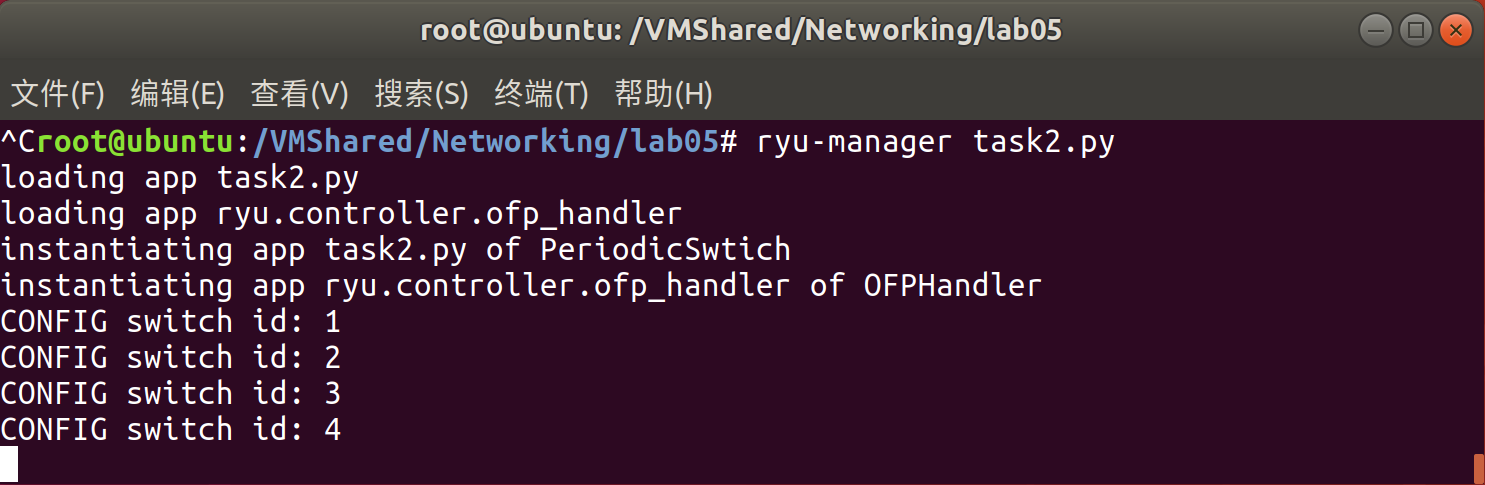
\includegraphics[width=0.6\linewidth]{idorder}
        \caption{交换机编号}\label{fig:idorder}
    \end{figure}

    使用下面的命令可以可视化地观察流信息\cite{gui},并启动控制器。
    \begin{lstlisting}[style=commandshell]
        ryu/ryu/app/gui_topology$ ryu-manager --observe-links gui_topology.py ../../../../lab05/task2.py\end{lstlisting}

    \begin{figure}[H]
        \centering
        \begin{minipage}{0.48\textwidth}
            \centering
            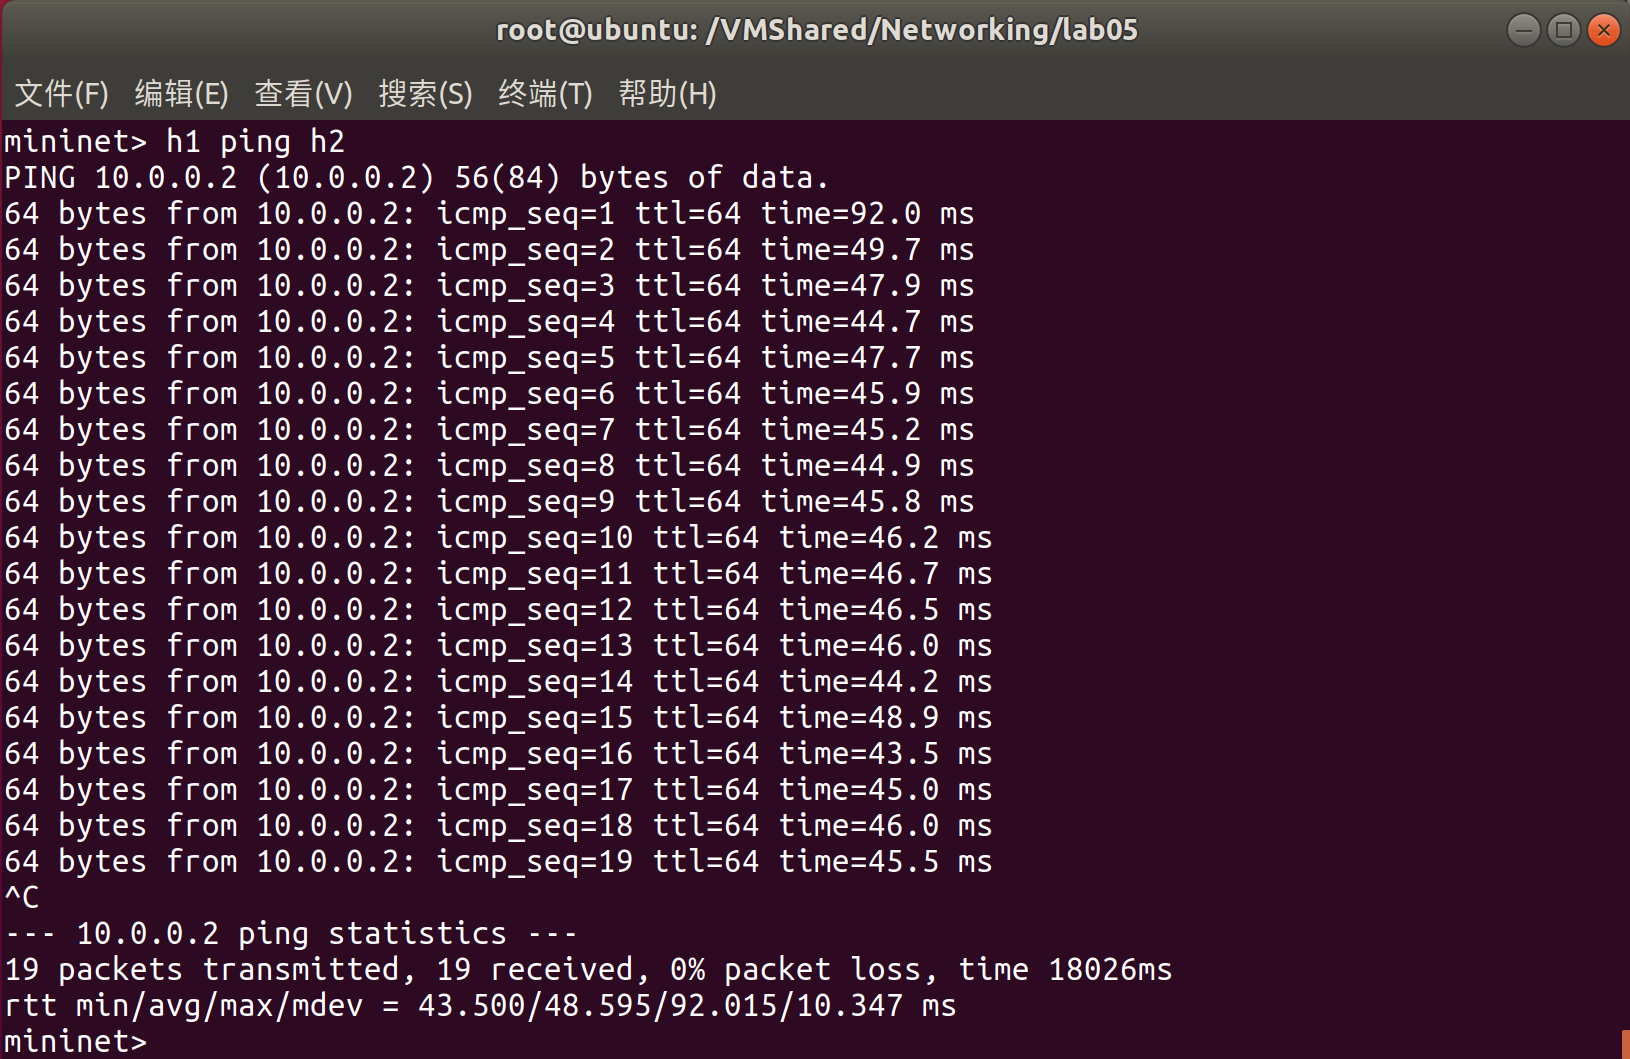
\includegraphics[width=\linewidth]{task2ping}
            \caption{测试连接}\label{fig:task2ping}
        \end{minipage}
        \begin{minipage}{0.48\textwidth}
            \centering
            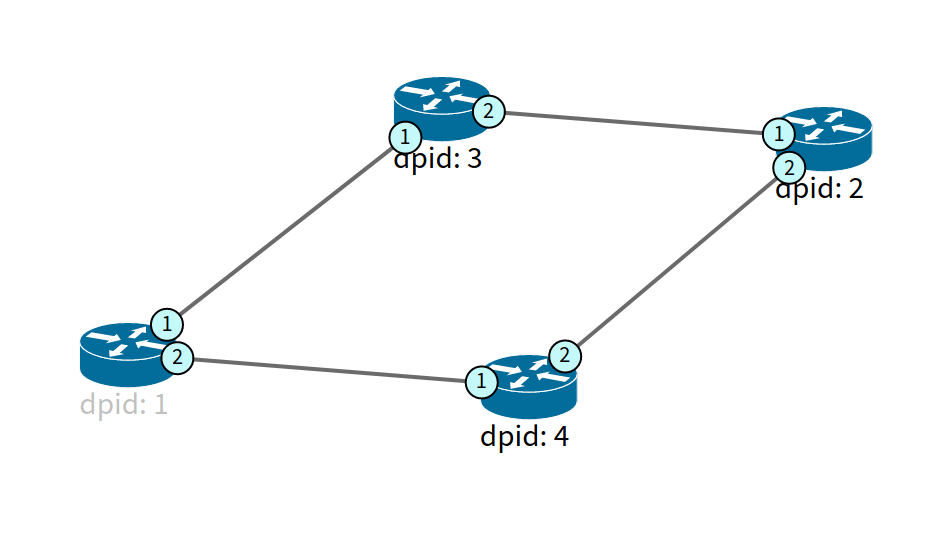
\includegraphics[width=\linewidth]{task2topo}
            \caption{\texttt{gui\_topology} 展示的拓扑结构}\label{fig:task2topo}
        \end{minipage}
    \end{figure}

    由图 \ref{fig:task2topo} 可见,可以通过定时切换 \verb"s1" 和 \verb"s2" 的输出端口,来达到切换链路的功能。切换为 \verb"3" $\rightarrow$ \verb"1" 采用上面的链路,切换为 \verb"3" $\rightarrow$ \verb"2" 采用下面的链路。由于有两个流会超时,但是临近的两个超时应当只改变一次端口状态,所以会设置一个状态变量用于避免不同步情况的设置延迟导致的丢包,如图 \ref{fig:pathstate} 所示。在图 \ref{fig:task2ping} 中可见是能够 \verb"ping" 通的。相关代码见附录 \ref{sec:per5}。

    \begin{figure}[H]
        \centering
        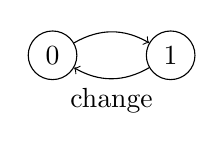
\begin{tikzpicture}
\node[draw,circle] (v1) at (0,0) {0};
\node[draw,circle] (v2) at (1.5,0) {1};
\draw[bend left,->]  (v1) edge (v2);
\draw[bend left,->]  (v2) edge node[below] {change}  (v1);
\end{tikzpicture}
        \caption{状态机}\label{fig:pathstate}
    \end{figure}

    \section{使用双路}
    Write an RYU controller that uses both paths to forward packets from h1 to h2.

\begin{quotation}
    \textbf{select}: Execute one bucket in the group. Packets are processed by a single bucket in the
group, based on a switch-computed selection algorithm (e.g. hash on some user-configured tuple or
simple round robin). All configuration and state for the selection algorithm is external to OpenFlow.
The selection algorithm should implement equal load sharing and can optionally be based on bucket
weights. When a port specified in a bucket in a select group goes down, the switch may restrict bucket
selection to the remaining set (those with forwarding actions to live ports) instead of dropping packets
destined to that port. This behavior may reduce the disruption of a downed link or switch.\cite{openflow13}
\end{quotation}



    \section{}
    Write an RYU controller that uses the first path (h1-s1-s3-s2-h2) for routing packets from h1 to h2 and uses the second path for backup. Specifically, when the first path experiences a link failure, the network should automatically switch to the second path without causing packet drop. (hint: consider using \verb"OFPGT_FF" (FF is short for ``fast failover'') to construct a group table)

    \begin{quotation}
        \textbf{fast failover}: Execute the first live bucket. Each action bucket is associated with a specific
port and/or group that controls its liveness. The buckets are evaluated in the order defined by the
group, and the first bucket which is associated with a live port/group is selected. This group type
enables the switch to change forwarding without requiring a round trip to the controller. If no buckets
are live, packets are dropped. This group type must implement a \emph{liveness mechanism}(see 6.5).\cite{openflow13}
    \end{quotation}

    \bibliography{ref}

    \appendix

    \section{定时切换代码}\label{sec:per5}

    \code{task2.py}

\end{document}